%import template
\documentclass[a4paper, landscape , 5pt]{scrartcl}

% use language german
\usepackage[T1]{fontenc}
\usepackage[utf8]{inputenc}
\usepackage[english, ngerman]{babel} % \selectlanguage{english} if  needed
\usepackage{lmodern} % use modern latin fonts

% format
\usepackage{geometry}
\geometry{top=0.8cm,left=0.4cm,right=0.4cm}
\textheight = 574pt

%autor
\usepackage{authblk}

%tabular
\usepackage{tabularx}

% math
\usepackage{amsmath}
\usepackage{amssymb}
\usepackage{amsfonts}
\usepackage{enumitem}

% graphic
\usepackage{graphicx}
\graphicspath{{graphic/}} 

%colors
% \usepackage{xcolor}

% Multi Columns
\usepackage{multicol}

% List indents
\usepackage{enumitem}
\setlist[itemize,2]{left=-1mm}

%compact items
\setlist{topsep=0pt, leftmargin=2mm, nolistsep}
\setlength{\parindent}{0cm}

%define header and footer
\usepackage{fancyhdr}
\pagestyle{fancy}

\fancyhead[RO]{\AUTHOR| \INSTITUTE}
\fancyhead[LO]{\TITLE}
\fancyfoot[RO]{FS 2025}
\renewcommand\headrulewidth{0pt}
\renewcommand\footrulewidth{0pt}
\renewcommand{\familydefault}{\sfdefault}
\headsep = -2pt
\footskip = 0pt


% Define Section Format
\usepackage{sectsty}
\usepackage{titlesec}
\usepackage[dvipsnames]{xcolor}

\titleformat{name=\section}[block]{\sffamily\small}{}{0pt}{\colorsection}
\titlespacing*{\section}{0pt}{0pt}{0pt}
\newcommand{\colorsection}[1]{%
	\colorbox{sectioncolor!80}{\parbox{0.98\linewidth}{\vspace{-3pt}\color{white}\ #1 \vspace{-6pt}}}}

% Define Subsection Format
\titleformat{name=\subsection}[block]{\sffamily\small}{}{0pt}{\colorsubsection}
\titlespacing*{\subsection}{0pt}{0pt}{0pt}
\newcommand{\colorsubsection}[1]{%
	\colorbox{subsectioncolor!80}{\parbox{0.98\linewidth}{\vspace{-3pt}\color{black}\ #1 \vspace{-6pt}}}}

% Define SubSubsection Format
\titleformat{name=\subsubsection}[block]{\sffamily\small}{}{0pt}{\colorsubsubsection}
\titlespacing*{\subsubsection}{0pt}{0pt}{0pt}
\newcommand{\colorsubsubsection}[1]{%
	\colorbox{subsubsectioncolor!60}{\parbox{0.98\linewidth}{\vspace{-3pt}\color{black}\ #1 \vspace{-6pt}}}}


%define color
\definecolor{sectioncolor}{HTML}{4B0082}
\definecolor{subsectioncolor}{HTML}{b366ff}
\definecolor{subsubsectioncolor}{HTML}{d6a1f7}
\definecolor{babyblue}{RGB}{173, 216, 230}
\definecolor{b}{RGB}{0, 115, 192 } %Default highlight color
\definecolor{p}{RGB}{0, 43, 54} %Dark page color
\definecolor{t}{RGB}{131, 148, 150} %Dark text color
\definecolor{darkgreen}{RGB}{0,150,0}
\definecolor{dkgreen}{rgb}{0,0.6,0}
\definecolor{gray}{rgb}{0.5,0.5,0.5}
\definecolor{mauve}{rgb}{0.58,0,0.82}
\definecolor{DarkPurple}{rgb}{0.4, 0.1, 0.4}
\definecolor{DarkCyan}{rgb}{0.0, 0.5, 0.4}
\definecolor{LightLime}{rgb}{0.3, 0.5, 0.4}
\definecolor{Blue}{rgb}{0.0, 0.0, 1.0}
\definecolor{h}{RGB}{1, 101, 163}

% Code ings
\usepackage{listings}
\usepackage{color}
\usepackage{beramono}
\usepackage{hyperref}
\hypersetup{
	colorlinks,
	linkcolor={black},
	citecolor={blue!50!black},
	urlcolor={blue!80!black}
}

\definecolor{bluekeywords}{rgb}{0,0,1}
\definecolor{greencomments}{rgb}{0,0.5,0}
\definecolor{redstrings}{rgb}{0.64,0.08,0.08}
\definecolor{xmlcomments}{rgb}{0.5,0.5,0.5}
\definecolor{types}{rgb}{0.17,0.57,0.68}

\lstdefinestyle{eclipse-style}{
	language=Java,
	showstringspaces=false,     
	basicstyle=\ttfamily\scriptsize,
	keywordstyle=\color{RoyalBlue}\ttfamily,
	stringstyle=\color{darkgreen}\ttfamily,
	commentstyle=\color{DarkPurple!60}\ttfamily,
	escapeinside={£}{£}, % latex scope within code      
	breaklines=true,
	breakatwhitespace=true,
	showspaces=false,
	showtabs=false,
	tabsize=2,
	morekeywords={length},
	numbers=none,
	numberstyle=\tiny\color{black},
	frame=none,
	aboveskip = 0em,
	belowskip = 0em
}
\lstset{
	style=eclipse-style
	% literate=  % Allow for German characters in lstlistings.
	% {Ö}{{\"O}}1
	% {Ä}{{\"A}}1
	% {Ü}{{\"U}}1
	% {ü}{{\"u}}1
	% {ä}{{\"a}}1
	% {ö}{{\"o}}1}
	}
	
	% Theorems \begin{mytheo}{title}{label}
\usepackage{tcolorbox}
\tcbuselibrary{theorems}
\newtcbtheorem[number within=section]{definiton}{Definition}%
{fonttitle=\bfseries}{def}
\newtcbtheorem[number within=section]{remember}{Merke}%
{fonttitle=\bfseries}{rem}
\newtcbtheorem[number within=section]{hint}{Hinweis}%
{fonttitle=\bfseries}{hnt}

% Front page
\newcommand{\AUTHOR}{Nicolas Caluori und Joëlle Schönenberger }
\newcommand{\INSTITUTE}{(L)Ostschweizer Fachhochschule}

%dotted rule
\usepackage{dashrule}
\usepackage{tikz}
\usetikzlibrary{decorations.markings}
\newcommand{\drule}[3][0]{
	\tikz[baseline]{\path[decoration={markings,
			mark=between positions 0 and 1 step 2*#3
			with {\node[fill, circle, minimum width=#3, inner sep=0pt, anchor=south west] {};}},postaction={decorate}]  (0,#1) -- ++(#2,0);}}


%no indentation
\setlength{\parindent}{0cm}


% no vertical distribution
% explanation: we copy the macro columnbreak to stdcolumnbreak
% we now redefine columnbreak to always fill up null space and then execute the standard columnbreak.
\let\stdcolumnbreak\columnbreak
\renewcommand\columnbreak{\vfill\null\stdcolumnbreak}


% DocInfo
\newcommand{\SUBJECT}{}
\newcommand{\TITLE}{Cheat Sheet Computernetze 2}

\begin{document}
	
	%import front page
	% \input{./front.tex}
	
	%do multicols
	\begin{multicols*}{5}
		\setlength{\columnseprule}{0.4pt}
		\footnotesize
		
		%import tableofcontents
		% \input{./tableofcontents.tex}
		
		\section{OSPF (IGP)}
		Equal Cost Multipath (ECMP) load balancing, fast convergence, widely used. Uses IP Port 89 on Layer 3. Uses 224.0.0.5 (all routers), 224.0.0.6 (all DR,BDR) \\
		\textbf{DR Election:} Highest interface priority → if tie, highest Router ID. Priority 0 = ineligible for DR/BDR. No preemption. BDR = same rules, second best candidate
		\subsection{Router Operation}
		\begin{enumerate}
			\item Establish neighbor adjacencies and exchange LSAs
			\item Build the Link-State Database (LSDB)
			\item Run Dijkstra's SPF algorithm:
			\begin{itemize}
				\item \textbf{Intra-area change:} SPF recalculation
				\item \textbf{Inter-area change:} No SPF needed — ABR handles updates
			\end{itemize}
			\item Build the routing table from SPF results
		\end{enumerate}
		\subsection{Areas}
		\begin{itemize}
			\item AS split into \textbf{areas} (sub-domains), each with a 32-bit Area ID (e.g., \textit{0.0.0.0} = Area 0)
			\item \textbf{Backbone Area (Area 0):} Core of the OSPF domain (must exist) Must connect to all other areas (directly or via virtual links), Must be contiguous (no disjointed segments), Should not contain end-user networks
			\item \textbf{Non-Backbone Areas:} Connect end users and local resources, All inter-area traffic must transit the backbone
		\end{itemize}
		\subsection{Router Types}
		\begin{itemize}
			\item \textbf{Area Border Router (ABR):} Connects two or more OSPF areas, must have 1 interface in backbone. 1 OSPF DB per Area
			\item \textbf{Internal Router:} All interfaces belong to the same area (non-backbone)
			\item \textbf{Backbone Router:} At least one interface in Area 0, Includes ABRs and routers internal to the backbone
			\item \textbf{AS Boundary Router (ASBR):} Connects to external AS/Network (e.g., BGP), Advertises external routes into OSPF, Can be in backbone or non-backbone area
		\end{itemize}
		\subsection{Design Rules}
		\begin{itemize}
			\item \textbf{Rule 1:} Backbone (Area 0) must be contiguous — no partitions allowed
			\item \textbf{Rule 2:} Every non-backbone area must connect to Area 0
		\end{itemize}
		
		\subsection{LSA Type Overview}
		\begin{itemize}
			\item \textbf{Type 1 – Router-LSA:} Sent by all routers, lists directly connected links (so all outgoing interfaces with state and cost) (intra-area only)
			\item \textbf{Type 2 – Network-LSA:} Sent by DR, lists all routers and DR in broadcast/multi-access network (intra-area only)
			\item \textbf{Type 3 – Summary-LSA:} Sent by ABRs, advertises networks from other areas, flooded in all the areas that are not "totally stubby" (inter-area)
			\item \textbf{Type 4 – ASBR-Summary:} Sent by ABRs, advertises path to ASBRs (inter-area)
			\item \textbf{Type 5 – AS-External-LSA:} Advertises external routes (e.g., BGP); flooded to all non-stub areas -> only normal areas
			\item \textbf{Type 7 – NSSA External:} Like Type 5 but used inside NSSA; converted to Type 5 by ABR
		\end{itemize}
		\subsection{Area Types (\{allowed LSA Types\})}
		{\setlength\multicolsep{1pt}%
			\begin{multicols}{2}
				\textbf{Standard (1,2,3,4,5)} Normal \\
				\textbf{Stub Area (1,2,3)}
				\begin{itemize}
					\item Blocks external LSAs (Type 5)
					\item ABR injects a default route (0.0.0.0)
					\item Supports LSA Types 1–3
				\end{itemize}
				
				\textbf{Totally Stubby Area (1,2):}
				\begin{itemize}
					\item Blocks external (Type 5) and summary (Type 3/4)
					\item Only allows default route from ABR
				\end{itemize}
				
				\textbf{Not-So-Stubby Area – NSSA (1,2,3,7):}
				\begin{itemize}
					\item Like stub area, but allows one ASBR inside
					\item External routes use LSA Type 7 (converted to Type 5 by ABR)
				\end{itemize}
				
				\textbf{Totally NSSA (1,2,7):}
				\begin{itemize}
					\item Like NSSA but blocks Type 3 so gets default route from ABR
				\end{itemize}
			\end{multicols}
		}
		\subsection{Packet Types}
		\begin{itemize}
			\item \textbf{Type 1 – Hello:}  
			Used to discover, maintain, and verify neighbors; forms adjacencies. Also for election of DR,BDR in broadcast networks. Contains network mask(of sending routers' interface), Hello interval(p2p,broadcast: default=10s), Options, Priority(for election), Router dead interval(default=40s), DR/BDR IP, Neighbors.
			
			\item \textbf{Type 2 – Database Description (DBD/DD):}  
			Exchange summaries of LSAs during adjacency formation (headers only). Contains Interface Max. MTU, Options, I/M/MS bits (Initial, More, Master-slave bit), DD Sequence num, LSA Header
			
			\item \textbf{Type 3 – Link State Request (LSR):}  
			Sent when a router needs specific LSAs listed in the DBD. Contains Link State Type (router/network), Link State ID, Advertising Router (sender address)
			
			\item \textbf{Type 4 – Link State Update (LSU):}  
			Used to flood new or updated LSAs. Contains Number of LSAs, full LSAs information
			
			\item \textbf{Type 5 – Link State Acknowledgment (LSAck):}  
			Confirms receipt of LSAs to ensure reliable flooding. For this you send LSAck or implicitly by sending LSU with same info back. Many acks may be grouped together to a single LSAck.
		\end{itemize}
		
		\subsection{Sub-Protocols}
		\begin{itemize}
			\item \textbf{Hello Protocol:}
			\begin{itemize}
				\item Used for neighbor discovery and parameter negotiation.
				\item Maintains logical adjacencies on P2P, P2MP, and virtual links.
				\item Elects DR/BDR on broadcast and NBMA networks.
				\item Continuously sends hello packets to maintain bidirectional connectivity; failure to receive = neighbor down (in agreed router dead interval at initialization)
			\end{itemize}
			
			\item \textbf{Database Sync Protocol:}
			\begin{itemize}
				\item Syncs LSDB using Database Description (DBD) packets with only LSA headers.
				\item Uses I-bit (initial), M-bit (more), and MS-bit (master/slave).
				\item \textbf{ExStart:} Bi-dir comm; highest Router-ID = master. Determine initial seq nr
				\item \textbf{Exchange:} Exchange of DBD packets (LSA headers).
				\item \textbf{Loading:} Missing LSAs are requested.
				\item \textbf{Full:} Databases fully synchronized.
			\end{itemize}
		\end{itemize}
		
		\subsection{OSPF Routing and ECMP}
		\begin{itemize}
			\item Each router runs Dijkstra per area; link cost = metric from LSAs (1–65535)
			\item OSPF perfers more specific match (CIDR) and if then still multiple: intra-area > inter-area > external
			\item Routes added to RIB/FIB based on computed next hops
			\item \textbf{ECMP:} Modified Dijkstra supports Equal-Cost MultiPath if multiple paths have same cost → routes added with multiple next-hops for load balancing
		\end{itemize}
		
		\subsection{OSPF Route Selection}
		\begin{itemize}
			\item \textbf{Intra-Area (O):} Source and dest in same area; routes from Type 1 and 2 LSAs
			\item \textbf{Inter-Area (O IA):} Source and dest in different areas within same AS; via Type 3 LSAs through backbone
			\item \textbf{External (E1/E2):} Dest outside AS; info injected by ASBR via redistribution
			\begin{itemize}
				\item \textbf{E1:} Total = external + internal OSPF cost
				\item \textbf{E2:} Only external cost (default)
			\end{itemize}
			\item \textbf{Preference order:} More specific route > Intra-area > Inter-area > E1 > E2
			\item \textbf{Cost calculation:} Cost = Reference Bandwidth(default 100 Mbps)/Interface Bandwidth
		\end{itemize}
		
		\section{IS-IS (IGP)}
		\subsection{CLNS - Connectionless Network Services}
		\begin{itemize}
			\item \textbf{CLNS:} ISO Layer 3 datagram service; supports \textbf{CLNP}, \textbf{ES-IS}, \textbf{IS-IS}.
			\item \textbf{CLNP:} Connectionless Network Protocol, similar to IP, used in ISO stack (EtherType 0xFEFE).
			\item \textbf{IS-IS:} Link-state routing protocol (Layer 3); forms adjacencies with ES-IS; designed for CLNP but extended (Integrated IS-IS) to support IP.
			\item \textbf{Integrated IS-IS:} Allows IP routing with IS-IS; used widely by service providers even without CLNP.
		\end{itemize}
		\subsection{NET Addressing (type of NSAP (Network Service Access Point) address)}
		\begin{itemize}
			\item \textbf{NET = Network Entity Title:} Unique router identifier in IS-IS
			\item \textbf{Format:} \textit{49.AAAA.BBBB.BBBB.BBBB.00}
			\item \textbf{49.AAAA...:} Area ID (variable length)
			\item \textbf{BBBB.BBBB.BBBB:} System ID (usually 6 bytes = unique router ID)
			\item \textbf{00:} N-Selector (NSEL) (always \textit{00} for routers)
			\item \textbf{System ID:} Must be unique per router (often based on lo-IP/MAC)
			\item Example: \textit{49.0001.1921.6800.1024.00} based on IP 192.168.1.24
			\item \textbf{Area ID:} Used for routing hierarchy (like OSPF areas)
		\end{itemize}
		\subsection{IS-IS Packet Types (all in L1 or L2)}
		\begin{itemize}
			\item \textbf{IIH (Hello):} Builds and maintains adjacencies; includes system ID, holding time, prio
			\begin{itemize}
				\item Built from 3 functions: \textbf{discover, build, maintain}
				\item \textbf{Interval:} 10s (default); DIS sends every 3.3s on LANs
				\item \textbf{Multiplier:} Missed Hello limit → Holdtime = Interval × Multiplier(default=3)
				\item \textbf{Multicast:}
				\begin{itemize}
					\item \textit{01-80-C2-00-00-14} (AllL1ISs)
					\item \textit{01-80-C2-00-00-15} (AllL2ISs)
				\end{itemize}
			\end{itemize}
			
			\item \textbf{LSP (Link State PDU):} Contains topology info including prefixes with costs; flooded throughout the area -> similar to OSPF LSA Type 1
			\item \textbf{CSNP (Complete SNP):} Sent by DIS; lists all known LSPs (used for database sync)
			\item \textbf{PSNP (Partial SNP):} Used to request missing LSPs or acknowledge received LSPs
			\item \textbf{IS-IS Packet Structure:} Common header + TLVs
		\end{itemize}
		\subsection{Router Types}
		\begin{itemize}
			\item \textbf{L1 Router:} Only within one area; no inter-area routing
			\item \textbf{L2 Router:} Backbone router; routes between areas
			\item \textbf{L1/L2 Router:} Acts as both; separates databases, redistributes between levels
		\end{itemize}
		\subsection{Broadcast/Multi-Access Links: DIS – Designated IS}
		\begin{itemize}
			\item Required on broadcast links (no DIS on p2p)
			\item Sends periodic \textbf{CSNPs} to ensure DB sync, creates \textbf{pseudonode LSP}
			\item No backup DIS in IS-IS
		\end{itemize}
		
		\subsubsection{DIS Election}
		\begin{itemize}
			\item 1. Highest interface priority (0–127) Ciso default = 64
			\item 2. Highest SNPA (MAC-Address!)
			\item \textbf{Preemption:} Enabled – higher prio router automatically takes ver the DIS Role
		\end{itemize}
		\subsection{Point-to-Point links (No DIS)}
		\begin{itemize}
			\item \textbf{CSNP:} Sent once at adjacency startup
			\item \textbf{LSP:} Advertises topology changes (link-state info)
			\item \textbf{PSNP:} Acknowledges received LSPs or requests missing ones
		\end{itemize}
		
		\subsection{Path Selection}
		\textbf{Path Selection Order (in IS-IS) - Lower Metric better:}
		\begin{enumerate}
			\item L1 intra-area routes
			\item L2 intra-area routes
			\item Leaked L2→L1 (internal metric)
			\item L1 external (external metric)
			\item L2 external (external metric)
			\item Leaked L2→L1 (external metric)
		\end{enumerate}
		\subsection{Level 1 Routing}
		\begin{itemize}
			\item Intra-area routing only (like OSPF intra-area)
			\item L1 routers use the closest L1/L2 router for inter-area traffic
			\item \textbf{L1/L2 routers:}
			\begin{itemize}
				\item Do \textbf{not} advertise L2 routes into the L1 area (unless route leaking is active)
				\item Set \textbf{Attached bit} to signal L2 connectivity to backbone
			\end{itemize}
			\item L1 routers install a \textbf{default route} to nearest L1/L2
			\item L1 area like OSPF Totally Stubby Area
			\item \textbf{Distribution Bit:} Set to 'up' (1) on L2→L1 leaks; blocks re-advertisement L1→L2.
			\item \textbf{Route-Leaking} injects a more specific route into L1 to improve routing
		\end{itemize}
		
		\subsection{Level 2 Routing}
		\begin{itemize}
			\item Routing between areas (inter-area)
			\item L1/L2 routers inject L1 routes into L2 topology
			\item L1 routes are redistributed into L2 with L1 metric preserved in L2 LSP
		\end{itemize}
		\subsection{IS-IS vs OSPF}
		\begin{tabular}{p{1.0cm} | p{1.5cm} | p{1.5cm}}
			\textbf{Feature} & \textbf{IS-IS} & \textbf{OSPF} \\
			\hline
			Layer & L2 (CLNS) & L3 (IP, proto 89) \\
			Encapsulation & No IP, uses TLVs & IP packets \\
			Hello Type & IIH & Hello packet \\
			Area Model & L1/L2 & Backbone + Areas \\
			Metric & Cost (default 10) & Cost (bandwidth) \\
			Router ID & System ID (6B) & 32-bit Router ID \\
			Adj. Types & L1, L2, L1/L2 & DR/BDR, P2P \\
			LSDB & Per level (L1/L2) & Per area \\
			Scaling & Large-scale ISP core & Enterprise/campus \\
			Routing Info & TLVs (flexible) & Fixed LSA types \\
		\end{tabular}
		\section{BGP (EGP)}
		\subsection{Config}
		\begin{itemize}
			\item \textbf{next-hop-self} fixing iBGP: neighbor (neighbor IP) next-hop-self (when overriding)
		\end{itemize}
		\subsection{BGP Sessions}
		\begin{itemize}
			\item Point-to-point adjacencies between BGP routers
			\item \textbf{iBGP:} Between routers in the same AS, AD=200, more trusted (lower security overhead)
			\item \textbf{eBGP:} Between routers in different ASes, AD=20, stricter policy enforcement
		\end{itemize}
		\subsection{Autonomous System Numbers (ASN)}
		\begin{itemize}
			\item Unique ID for each AS; required for Internet routing with BGP
			\item Private ranges:
			\begin{itemize}
				\item 64\,512–65\,535 (legacy 16-bit)
				\item 4\,200\,000\,000–4\,294\,967\,294 (32-bit)
			\end{itemize}
		\end{itemize}
		
		\subsection{BGP Peering / Neighbors}
		\begin{itemize}
			\item Two routers with a BGP TCP session (port 179) are called peers or neighbors
			\item Each BGP router is a \textbf{BGP speaker}
			\item BGP exchanges routing info between ASes (loop-free, policy-based)
			\item Supports CIDR, route aggregation; decisions based on policies/rules
		\end{itemize}
		
		\subsection{Path Attributes}
		\begin{itemize}
			\item Used for route control and policy enforcement
			\item \textbf{Well-known mandatory:} Always present (e.g., AS-Path, Origin, Next Hop)
			\item \textbf{Well-known discretionary:} Optional but recognized by all (e.g., Local Pref, Atomic Aggregate)
			\item \textbf{Optional transitive:} Passed between ASes (e.g., Community, Aggregator)
			\item \textbf{Optional non-transitive:} Not passed across ASes (e.g., MED, Weight, Originator ID, Cluster ID/List)
			\item \textbf{NLRI:} Routing table info: prefix, prefix length, and associated path attributes
		\end{itemize}
		
		\subsection{Loop Prevention}
		\begin{itemize}
			\item BGP uses \textbf{AS-Path} (list of ASNs) to detect loops
			\item If a router sees its own ASN in a received route, it discards it
			\item \textbf{AS-Override:} Allows reuse of same ASN across different customer sites (e.g., Swisscom); rewrites ASN to avoid loop detection
		\end{itemize}
		
		\subsection{BGP Messages}
		\begin{itemize}
			\item \textbf{OPEN:} Establishes session; includes version, ASN, Hold Time, BGP Identifier, optional params
			\begin{itemize}
				\item \textbf{Hold Time:} Heartbeat in seconds (default 180s, Cisco), reset by KEEPALIVE/UPDATE; 0 = session down
				\item \textbf{BGP Identifier:} 32-bit Router-ID, manually set or highest loopback/active IP; used for loop prevention
			\end{itemize}
			\item \textbf{KEEPALIVE:} Sent every 1/3 of Hold Time (default 180s); ensures neighbor liveness (BGP doesn’t rely on TCP keepalive)
			\item \textbf{UPDATE:} Advertises new routes, withdraws old ones, or both; includes NLRI (prefix + path attributes); can act as KEEPALIVE
			\item \textbf{NOTIFICATION:} Sent on session error (e.g. hold timer expired); terminates session immediately
		\end{itemize}
		
		\subsection{BGP Network Statements}
		\begin{itemize}
			\item \textbf{Purpose:} Advertise specific prefixes to BGP peers (does not activate interfaces)
			\item Prefix must exist exactly in the RIB (from static, connected, or learned route)
			\item Attributes (e.g., origin, next-hop, MED) depend on how the route exists in RIB
			\item BGP advertises only the best path for a prefix to peers, even if multiple exist
		\end{itemize}
		
		\subsection{Best Path Calculation}
		\begin{itemize}
			\item BGP maintains all received paths per prefix but advertises only the best one
			\item Best path is installed in RIB; recalculated on:
			\begin{itemize}
				\item Next-hop reachability change
				\item Interface failure to eBGP peer
				\item Redistribution change
				\item New/withdrawn path received
			\end{itemize}
			\item \textbf{Influence:}
			\begin{itemize}
				\item Outbound BGP policy → inbound traffic behavior
				\item Inbound BGP policy → outbound traffic behavior
			\end{itemize}
		\end{itemize}
		
		\subsubsection*{BGP Best Path Selection (in order):}
		\begin{enumerate}
			\item Prefer highest \textbf{Weight} (Cisco-specific, local to router)
			\item Prefer highest \textbf{Local Preference} (global within AS)
			\item Prefer routes \textbf{originated by the router} (only small i in path, NH 0.0.0.0)
			\item Prefer \textbf{shorter AS path} (only length is compared) 
			\item Prefer \textbf{lowest origin type:} IGP < EGP < Incomplete (I on origin)
			\item Prefer \textbf{lowest MED} (Multi-Exit Discriminator) (also called metric)
			\item Prefer \textbf{external (EBGP)} over \textbf{internal (IBGP)}
			\item For iBGP: prefer path with \textbf{lowest IGP metric} to next-hop
			\item For eBGP: Prefer \textbf{oldest} (more stable) path
			\item Prefer \textbf{lowest BGP router ID}
			\item Prefer path from \textbf{lowest neighbor IP address}
		\end{enumerate}
		
		\subsection{Route Filtering}
		\begin{itemize}
			\item Filters control which routes are received/advertised
			\item Used for security, traffic shaping, memory optimization
			\item Tools: \textbf{prefix-list} (IP), \textbf{filter-list} (AS-path), \textbf{route-map} (flexible match/set)
		\end{itemize}
		
		\subsection{BGP Communities}
		\begin{itemize}
			\item 32-bit optional, transitive tag (e.g. \textit{ASN:value}, \textit{65000:100})
			\item Used to mark routes for policy control across ASes
			\item Can be added, modified, or removed at each hop
		\end{itemize}
		
		\subsection{iBGP Scalability}
		\begin{itemize}
			\item iBGP does not re-advertise routes between iBGP peers → full mesh required (cause no loop prevention)
			\item Session count = $n(n{-}1)/2$ (e.g., 5 routers = 10 sessions, 10 = 45)
		\end{itemize}
		
		\subsubsection*{Route Reflectors (RR)}
		\begin{itemize}
			\item Solves iBGP full-mesh scaling by allowing selective route reflection
			\item Clients only peer with RR; unaware they’re clients
			\item \textbf{RR Rules:}
			\begin{enumerate}
				\item From \textbf{non-client} → advertise to \textbf{clients only}
				\item From \textbf{client} → advertise to \textbf{all} (clients \& non-clients)
				\item From \textbf{eBGP peer} → advertise to \textbf{all} (clients \& non-clients)
			\end{enumerate}
			\item Only the RR needs special config - clients remain unaware of route reflection. This eliminates the need for full iBGP mesh.
		\end{itemize}
		
		\subsection{Peering vs. Transit}
		\begin{itemize}
			\item \textbf{Transit:} ISP provides full reachability (paid relationship)
			\item \textbf{Peering:} ISPs exchange selected routes; equal relationship, usually unpaid
			\item \textbf{AS Path Filtering:} to avoid getting transit:	 ip as-path access-list 10 permit \^ \$
		\end{itemize}
		
		\subsection{Internet Exchange Point (IXP)}
		\begin{itemize}
			\item Facility where networks exchange traffic via BGP peering
			\item Reduces transit costs, latency, and offloads upstream links
		\end{itemize}
		
		\subsubsection*{Public Peering}
		\begin{itemize}
			\item Members peer via shared switch fabric and a \textbf{route server}
			\item Route server distributes routes but stays out of data path (NEXT\_HOP unchanged)
			\item Minimal policy control; one BGP session to route server
			\item Simplified setup (one legal contract)
		\end{itemize}
		
		\subsubsection*{Private Peering}
		\begin{itemize}
			\item Direct BGP sessions between two parties (1:1)
			\item May use public or private interconnects
			\item Full policy control per neighbor
			\item Requires one session and legal contract per peer
		\end{itemize}
		
		\textbf{Examples:} Equinix, SwissIX (non-profit)
		
		\subsection{Enterprise Connectivity Options}
		\begin{itemize}
			\item \textbf{Single-Homed:} One ISP, one link (BGP or static); simple but no redundancy
			\item \textbf{Dual-Homed:} One ISP, two links (or routers); redundancy within same provider
			\item \textbf{Multihomed:} Multiple ISPs; improved redundancy and routing control, but avoid being a transit — advertise only customer-owned prefixes
			\item \textbf{Dual-Multihomed:} Multihomed, but two links per ISP
		\end{itemize}
		
		\subsubsection*{Traffic Engineering (TE)}
		\begin{itemize}
			\item \textbf{Outbound TE (Local Pref):} Set higher local pref to prefer exit path; affects outbound traffic; highest wins
			\item \textbf{Inbound TE (MED):} Signal entry preference with MED; lowest wins; only works if peer honors it
			\item \textbf{Inbound TE (AS-Path Prepending):} Add own ASN multiple times on backup path; shortest AS-path wins
			\item \textbf{TE Limitation:} AS controls outbound (e.g. local pref); inbound control limited — ISPs may ignore MED
			\item \textbf{TE with Aggregate:} Prefer primary ISP with summarized routes; advertise specific prefixes on backup for failover
			\item \textbf{Aggregate Impact:} Longest-match wins → specific prefixes may steer traffic to alternate ISP; avoid provider-owned aggregates
		\end{itemize}
		
		\subsection{RPKI – Resource Public Key Infrastructure}
		\begin{itemize}
			\item Framework to validate that a prefix is legitimately originated by a specific ASN
			\item Prevents route hijacking and accidental mis-originations (route leaks)
			\item RPKI validates origin only — not the AS-path
		\end{itemize}
		
		\subsubsection*{Key Components}
		\begin{itemize}
			\item \textbf{Trust Anchors (TAs):} Root CAs of the 5 RIRs; issue certs for resource holders
			\item \textbf{ROA – Route Origin Authorization:} Digitally signed object that authorizes ASN to announce a prefix (contains AS, prefix that AS can originate, max prefix length)
			\item \textbf{RPKI Validators:} Software that downloads, verifies, and stores Validated ROA Payloads (VRPs)
		\end{itemize}
		
		\subsubsection*{RPKI Validation States}
		\begin{itemize}
			\item \textbf{Valid:} Prefix + ASN match ROA
			\item \textbf{Invalid:} Prefix found, but ASN mismatch or prefix too long
			\item \textbf{Not Found / Unknown:} No matching ROA
		\end{itemize}
		
		\subsubsection*{Validator Details}
		\begin{itemize}
			\item Use TALs (Trust Anchor Locators) to fetch data from RIRs
			\item Validate cryptographic signatures (via X.509 certs with RFC 3779)
			\item Outputs VRPs; invalid objects are discarded
			\item Update frequency: >=24h (recommended), ~30–60min (practice)
			\item RRDP (RFC 8182) replacing rsync (uses HTTPS)
		\end{itemize}
		
		\subsection{BGP Monitoring}
		Event tracking, BGP hijack detection, Route leak detection, RPKI status check, Reachability tracking, AS path change tracking, AS path visualization
		
		\section{Network Design}
		\textbf{Pillars:} Scalability, Speed, Availability, Security, Manageability -> overall Cost
		\subsection{Availability Concepts (most important requirement)}
		\begin{itemize}
			\item \textbf{MTBF:} Mean Time Between Failures, \textbf{MTTR:} Mean Time to Repair
			\item $A=\frac{\textit{MTBF}}{\textit{MTBF} + \textit{MTTR}}$ MTBF combined: $\sum \frac{1}{\frac{1}{\textit{MTBF}_n}}$ parallel: $\textit{MTBF} \cdot \frac{3}{2}$
			\item Lower MTTR + higher MTBF = more availability
		\end{itemize}
		
		\subsection{Redundancy}
		\begin{itemize}
			\item Adds reliability, decreases MTBF but increases MTTR and complexity
			\item Balance: resilience vs. manageability
			\item \textbf{Backup Paths:} Duplicate devices/links on primary path, build extra links for redundancy, consider backup link capacity, consider failover speed
			\item \textbf{Load Balancing:} ECMP, EtherChannel, Port-Channel
		\end{itemize}
		
		\subsection{Hierarchical Design}
		\begin{itemize}
			\item \textbf{Access:} Connect end devices, high port count, port security, L2, QoS marking
			\item \textbf{Distribution:} L3, policy control, HSRP/VRRP, loop protection, small fault domain
			\item \textbf{Core:} High-speed backbone, L3 only, no policy, scalable/redundant, no security
			\item \textbf{Collapsed Core:} Combines Core + Distribution (small/medium networks)
		\end{itemize}
		
		\subsection{Flat Design}
		\begin{itemize}
			\item Any-to-any; small networks, MPLS/LAN setups
			\item Lacks scalability and control
		\end{itemize}
		
		\subsection{Fabric Design}
		\begin{itemize}
			\item Modern design using \textbf{Underlay/Overlay}
			\item Underlay = transport (e.g., IP, MPLS)
			\item Overlay = logical virtual topology (e.g., EVPN)
		\end{itemize}
		
		\subsection{Enterprise Campus}
		\begin{itemize}
			\item 100s/1000s of users, multiple buildings, one physical location
			\item Multiple interconnected LANs, connected via Ethernet and Wireless
		\end{itemize}
		
		\subsection{FHRP – First Hop Redundancy Protocols}
		\begin{itemize}
			\item Ensures default gateway is always reachable, PCs can only have one
			\item Enables fast failover during router failure
			
			\item \textbf{VRRP – Virtual Router Redundancy Protocol (Multivendor):} Shared virtual IP, real MACs per router, Master router handles forwarding
			
			\item \textbf{HSRP – Hot Standby Router Protocol (Cisco):} Shared virtual IP + virtual MAC, One active, others in standby -> faster
			
			\item \textbf{GLBP – Gateway Load Balancing Protocol (Cisco):} Load balancing + redundancy, Shared virtual IP + multiple virtual MACs, \underline{ Roles:} \textbf{AVG:} Answers ARP and sends virtual MAC addresses of AVFs \textbf{AVF:} Forwards traffic
			
		\end{itemize}
		
		\subsection{Data Center Designs}
		\begin{itemize}
			\item \textbf{ToR - Top of Rack:} switches per rack, less cabling, easy expansions/exchanges per 'rack', scalable glass fiber, ideal for high service density (full racks). \underline{But} more switches, more ports, more L2 Srv-2-Srv traffic, more STP to be managed
			\item \textbf{EoR - End of Row:} 1 switch per row, less switches, higher utilization of ports, switches all at one place, better L2 availability between racks. \underline{But} more cabling
		\end{itemize}
		
		\subsection{Traffic Directions}
		\begin{itemize}
			\item \textbf{North–South:} Between external networks (client-server, in/out DC)
			\item \textbf{East–West:} Within DC (e.g., server-server, storage)
		\end{itemize}
		
		\subsection{Three-Tier DC}
		\begin{itemize}
			\item Access – Aggregation – Core (like Hierarchical)
			\item Optimized for North–South traffic
			\item Not ideal for East–West communication
		\end{itemize}
		
		\subsection{Leaf-Spine Architecture}
		\begin{itemize}
			\item Two-tier: Leaf switches (access) connect to Spines (core)
			\item High performance, low latency
			\item Scalable, ideal for East–West traffic
		\end{itemize}
		\section{Multicast}
		\textbf{Use Cases:}  
		\textbf{1-to-Many:} Streaming, software updates, music-on-hold  
		\textbf{Many-to-Many:} Gaming, VR, stock data, group chat  
		
		\textbf{Benefits:} Efficient bandwidth, lower server/CPU load, no redundancy, supports multipoint apps  
		
		\textbf{Properties:}  
		UDP-based (no delivery guarantee, congestion control, or ordering)  
		Apps must handle drops, duplicates, out-of-order packets  
		
		\textbf{Source:} Sends to group IP; doesn't need to join  
		\textbf{Receiver:} Must explicitly join group to receive traffic 
		
		\subsection{Multicast Address Ranges}
		\begin{itemize}
			\item \textbf{224.0.0.0 – 224.0.0.255:} Link-local, TTL = 1 (not forwarded by routers)
			\item \textbf{224.0.1.0 – 224.0.1.255:} Reserved by IANA, routable
			\item \textbf{232.0.0.0 – 232.255.255.255:} Source-Specific Multicast (SSM)
			\item \textbf{239.0.0.0 – 239.255.255.255:} Administratively scoped (private multicast space)
		\end{itemize} 
		
		\subsection{Broadcast Basics}
		\begin{itemize}
			\item \textbf{L2 (Bridging):} MAC ffff.ffff.ffff; switches flood to all ports in VLAN
			\item \textbf{L3 (Routing):}
			\begin{itemize}
				\item 255.255.255.255: local broadcast, not routed
				\item Directed broadcast (e.g. 10.1.1.255): can be routed if enabled
			\end{itemize}
			\item L3 routes between subnets; L2 floods within same subnet
		\end{itemize}
		
		\subsection{L2 Multicast: MAC Mapping}
		\begin{itemize}
			\item \textbf{Step 1 – Get IP:} Example multicast IP address: \textit{239.5.5.5}
			\item \textbf{Step 2 – Convert to Binary:} \\
			\textit{239.5.5.5} = 11101111.00000101.00000101.00000101 
			→ Take only the last 23 bits: 00000101.00000101.00000101
			\item \textbf{Step 3 – Map to MAC Prefix:}  
			Use fixed MAC multicast prefix: 0100.5E
			→ Map last 23 bits to: 0100.5E.05.05.05
			\item \textbf{Step 4 – Final MAC Address:}  
			0100.5E05.0505
		\end{itemize}
		
		\subsection{IGMP – Internet Group Management Protocol (Host to first-hop-router)}
		\textbf{Purpose:} Manages group membership for IPv4 multicast on each segment
		\textit{}
		\begin{itemize}
			\item \textbf{IGMPv1}
			\begin{itemize}
				\item Basic join via query-response mechanism
				\item No way for a host to leave a group explicitly
				\item Router sends general membership queries every 60s to \textit{224.0.0.1}
				\item If no report is received, router removes group after timeout
				\item Receiver has no knowledge of the multicast source
			\end{itemize}
			
			\item \textbf{IGMPv2}
			\begin{itemize}
				\item Adds \textit{Leave Group} message (faster pruning of unused traffic)
				\item General queries to \textit{224.0.0.1} every 125s 'Any hosts interested in any groups?'
				\item Supports \textit{Group-Specific Queries} e.g. when someone leaves group ('anyone still interested in group xy?'), reducing broadcast overhead
				\item Still source-agnostic: receivers don’t know who the source is
			\end{itemize}
			
			\item \textbf{IGMPv3}
			\begin{itemize}
				\item Adds \textit{source filtering} (Include/Exclude lists)
				\item Enables Source-Specific Multicast (SSM) – receiver requests traffic only from selected source(s), no need for Rendezvous Point (RP) anymore
				\item Adds support for application-level access control and filtering
				\item Can also be used in ASM (Any Source Multicast), but mainly with SSM
			\end{itemize}
		\end{itemize}
		
		\subsection{IGMP Snooping}
		\begin{itemize}
			\item Without snooping: multicast = broadcast on VLAN
			\item With snooping: switch listens to IGMP messages and builds a forwarding table
			\item Default: snooping is enabled; switch needs IGMP Query to operate
		\end{itemize}
		
		\subsection{Reverse Path Forwarding (RPF)}
		\begin{itemize}
			\item \textbf{RPF Check:} To avoid loops, verifies that a multicast packet arrives on the interface that a unicast packet destined for the multicast source would be forwarded out of. 
		\end{itemize}
		
		\subsection{Rendezvous Point (RP)}
		\begin{itemize}
			\item Used in Shared Tree (\textit{*,G}) setups with PIM-SM
			\item RP acts as the common meeting point for sources and receivers
			\item RPF check is performed toward the RP (not the source)
			\item Once the source is known, routers may switch to a Source Tree (\textit{S,G})
		\end{itemize}
		
		\subsection{Shared Tree vs. Source-Based Tree}
		\textbf{Shared Tree (*,G):}
		\begin{itemize}
			\item IGMP host sends a membership report (IGMP Join)
			\item Router adds \textit{(*,G)} entry to multicast routing table
			\item \textit{*} means 'any source' — source is unknown/unspecified
		\end{itemize}
		
		\textbf{Source-Based Tree (S,G):}
		\begin{itemize}
			\item Built when router receives an \textit{(S,G)} join/report from IGMP host
			\item \textit{S} = known multicast source; \textit{G} = group
			\item Router adds \textit{(S,G)} to mroute table once source is known
		\end{itemize}
		
		\subsection{PIM – Protocol Independent Multicast (only between routers)}
		\begin{itemize}
			\item Relies entirely on the unicast routing table (RIB) for multicast forwarding decisions
			\item Protocol-independent: works with static routes, OSPF, IS-IS, etc.
		\end{itemize}
		
		\subsection{PIM-DM – Dense Mode (no RP)}
		\textbf{Push Model}: Floods multicast traffic to all interfaces; then prunes where no receivers exist.
		
		\begin{itemize}
			\item \textbf{1. Flooding:} Source sends traffic → forwarded out all multicast-enabled links using unicast RIB
			\item \textbf{2. Distribution Tree:} Initially includes entire network (shared tree rooted at source)
			\item \textbf{3. Prune Messages:} Routers without interested receivers send prunes upstream to remove themselves from the tree
			\item \textbf{4. State Maintenance:} Routers track source, receivers, interfaces to forward/prune per group
		\end{itemize}
		
		\subsection{PIM-SM – Sparse Mode (ASM, SSM)}
		\textbf{Pull Model:} Multicast traffic is only sent where requested. Works with IGMP to detect interested receivers and uses unicast routing for forwarding.
		
		\begin{itemize}
			\item \textbf{1. Join/Prune:} Routers send explicit join/prune messages to request or stop receiving multicast for group (G) to other routers
			\item \textbf{2. Forwarding:} Routers only forward multicast packets for group (G) on interfaces from which explicit joins were received
		\end{itemize}
		
		\subsection{ASM – Any Source Multicast (How it works with RP)}
		\begin{itemize}
			\item Works with \textbf{IGMPv1} or \textbf{IGMPv2} → receiver does not know the source
			\item Receiver sends \textit{IGMP Join (*,G)} to its first-hop router
			\item First-hop router forwards \textit{PIM Join (*,G)} hop-by-hop toward the Rendezvous Point (RP)
			\item RP acts as a common meeting point for sources and receivers
			\item Sources send multicast traffic to the RP via a \textit{PIM Register} tunnel
			\item All routers in the multicast domain must know the RP location
		\end{itemize}
		
		\subsection{SSM – Source Specific Multicast}
		\begin{itemize}
			\item Receiver subscribes using \textbf{IGMPv3}, providing both source (S) and group (G) to the first-hop router
			\item No Rendezvous Point (RP) required → \textbf{PIM-SSM builds only (S,G)} Shortest Path Trees (SPT)
			\item \textbf{No shared tree (*,G)} model used; SSM is source-directed
			\item IANA reserved \textit{232.0.0.0/8} for SSM in IPv4
			\item Join messages are forwarded hop-by-hop toward the source to establish forwarding path
			\item Uses unicast routing table (RPF) to maintain loop-free delivery
		\end{itemize}
		
		\subsection{PIM Sparse-Dense Mode}
		\begin{itemize}
			\item \textbf{PIM Sparse Mode:} Pull model – multicast traffic is forwarded only on request
			\item \textbf{PIM Dense Mode:} Push model – traffic is flooded everywhere, then pruned
			\item \textbf{Sparse-Dense Mode:} Supports both modes per multicast group; choice depends on RP availability
		\end{itemize}
		
		\subsection{PIM-DM vs. PIM-SM}
		PIM is protocol-independent: it relies on the unicast routing table for RPF checks and to forward joins toward the source or Rendezvous Point (RP).
		
		\noindent\begin{minipage}{\linewidth}
			\setlength\multicolsep{1pt}%
			\begin{multicols}{2}
				\begin{itemize}
					\item \textbf{PIM Dense Mode (DM)}
					\item"Push" model
					\item Floods multicast traffic throughout the network
					\item Prunes back where traffic unwanted
				\end{itemize}
				
				\columnbreak
				
				\begin{itemize}
					\item \textbf{PIM Sparse Mode (SM)}
					\item "Pull" model
					\item Traffic sent only on request
					\item Requires explicit \textit{Join} messages
				\end{itemize}
			\end{multicols}
		\end{minipage}
		\vspace*{-\baselineskip} % remove bottom space if needed
		
		\textbf{Usage Recommendation:}
		\begin{itemize}
			\item \textbf{Dense Mode:} Best for small or tightly scoped networks where most devices need multicast
			\item \textbf{Sparse Mode:} Preferred for large-scale or distributed environments where multicast receivers are few or spread out
		\end{itemize}
		
		\section{VXLAN}
		\textbf{Issues of L2:} STP, Max amount of VLANs (4094), Large MAC Address tables
		\begin{itemize}
			\item \textbf{VXLAN (Virtual Extensible LAN):} Tunnels Ethernet (Layer 2) over IP using MAC-in-UDP encapsulation (Port 4789). For flexible and scalable network segmentation.
			\item \textbf{VNID (VXLAN Network Identifier):} 24-bit identifier (up to 16 million segments) that defines the VXLAN broadcast domain.
			\item \textbf{VTEP (Virtual Tunnel Endpoint):} Device (switch, router, or host) responsible for encapsulating/de-encapsulating VXLAN traffic.
			\item \textbf{NVE (Network Virtual Interface):} Logical interface on a VTEP used for VXLAN tunnel operations.
		\end{itemize}
		
		\subsection{Tunnel}
		\begin{itemize}
			\item VXLAN establishes IP tunnels between VTEPs to extend Layer 2 networks across Layer 3 boundaries.
			\item VXLAN enables both L2 and L3 VPN functionality in overlay networks.
			\item VXLAN traffic is encapsulated in UDP (default port: \textit{4789}).
		\end{itemize}
		
		\subsection{Frame Format}
		\begin{itemize}
			\item Ethernet frame $\rightarrow$ VXLAN Header $\rightarrow$ UDP $\rightarrow$ Outer IP Header.
			\item The VXLAN header contains the 24-bit VNID and flags.
			\item Outer headers allow Layer 2 frames to traverse IP underlay networks.
		\end{itemize}
		
		\subsection{Virtual Network Identifier (VNI)}
		\begin{itemize}
			\item 24-bit VXLAN Network Identifier uniquely defines VXLAN segments.
			\item Replaces traditional VLAN IDs (12-bit), enabling ~16 million logical segments.
			\item Used by VTEPs to map traffic into corresponding Layer 2 domains.
		\end{itemize}
		
		\subsection{VXLAN Tunnel Endpoint (VTEP)}
		\begin{itemize}
			\item Connects the overlay (VXLAN) and underlay (IP) networks.
			\item \textbf{Types:}
			\begin{itemize}
				\item \textbf{Software VTEP:} Located on hypervisors using virtual switches.
				\item \textbf{Hardware VTEP:} Located on routers/switches with ASICs for performance.
			\end{itemize}
			\item \textbf{Interfaces:}
			\begin{itemize}
				\item \textbf{VTEP IP Interface:} Connects to the underlay network and handles encapsulation.
				\item \textbf{VNI Interface:} Virtual interface per segment (like SVI); handles segregation of Layer 2 domains.
			\end{itemize}
		\end{itemize}
		
		\subsection{MAC Address learning}
		\begin{itemize}
			\item \textbf{On control plane:} happens proactively, \textbf{on data plane:} ad-hoc with flooding
			\item Each VTEP maintains a VXLAN mapping table linking destination MAC addresses to remote VTEP IPs.
			\item \textbf{Learning via ARP:}
			\begin{enumerate}
				\item Host H1 sends ARP request, switches learn H1's MAC.
				\item ARP request is flooded to H2.
				\item H2 responds; switches learn H2's MAC.
			\end{enumerate}
			\item \textbf{Learning Methods:}
			\begin{itemize}
				\item \textbf{Static VXLAN:} Manual MAC-to-VTEP mappings. Doesn’t scale well; BUM traffic is inefficient.
				\item \textbf{Multicast VXLAN:} VTEPs join multicast groups per VNI. Scales better, offloads BUM replication. 20+ VTEPs = there is too much traffic, doesn't scale well
				\item \textbf{MP-BGP EVPN:} Modern solution using BGP as control plane. Dynamically learns MAC/IP info.
			\end{itemize}
		\end{itemize}
		
		\section{EVPN}
		Overcome flood-and-learn limitations, doesn't rely on data plane learning, utilizes robust control plane MP-BGP, works with different encapsulation techniques (VXLAN, MPLS), excellent scalability, l2 and l3 Support.
		
		\subsection{MP-BGP EVPN (Multiprotocol BGP for Ethernet VPN)}
		\begin{itemize}
			\item Enables protocol-based VTEP discovery and host reachability via control-plane learning
			\item Reduces flooding by replacing data-plane learning
			\item Extends BGP with multiprotocol capabilities (AFI/SAFI)
			\item Uses \textit{MP\_REACH\_NLRI} and \textit{MP\_UNREACH\_NLRI} for route advertisement and withdrawal
		\end{itemize}
		
		\subsection{EVPN Route Types}
		
		\textbf{Type 2 – Host Advertisement:} Advertises host MAC (mandatory), optionally IP, along with L2VNI and optionally L3VNI. Used for MAC learning, ARP suppression, and host mobility. Sent when host connects to VTEP.
		
		\textbf{Type 5 – Subnet Advertisement:} Advertises IP prefix + prefix length with L3VNI. Used for inter-subnet routing. VTEP redistributes connected/static/dynamic IP routes. Additional attributes: L3VNI, extended communities.
		
		\subsection{Host Deletion \& Move}
		
		\textbf{Host Deletion:} When a host detaches, its ARP (default: 1500s) and MAC entry (default: 1800s) time out on the VTEP. Upon aging, the VTEP withdraws the host’s MAC/L2VNI and IP/L3VNI advertisements.
		
		\textbf{Host Move:} When a host moves to a new VTEP, the new VTEP advertises updated reachability with a higher move sequence number. The old VTEP withdraws its entry, completing the migration.
		
		\subsection{Route Distinguisher (RD) vs. Route Target (RT)}
		\begin{itemize}
			\item \textbf{Route Distinguisher (RD):}
			Uniquely identifies VPN routes — allows same IP prefix to be used in different VPNs. Can be IPv4 or ASN 
			\textit{Used to make routes unique in BGP (VPNv4/v6).} Forms VPNv4 NLRI: \textit{RD:IPv4 prefix} 
			
			\item \textbf{Route Target (RT):}
			Controls route import/export between VRFs.
			\textit{Used as extended BGP community.}
			
			\item \textbf{How RTs Work:}
			\begin{itemize}
				\item A route is tagged with an RT when advertised by BGP.
				\item Other VRFs import the route if the RT matches their import policy.
				\item Allows overlapping or shared connectivity between tenants (e.g., shared services).
			\end{itemize}
			
			\item \textbf{Format:}
			Typically in the form \textit{ASN:nn} or \textit{IP:nn}, e.g., \texttt{65000:100}, \texttt{1:10}
			
			\item \textbf{Multiple RTs can be used:}
			A route can have multiple RTs for flexible policies (e.g., one RT for VPN, another for shared services)
		\end{itemize}
		
		\section{EVPN (Ethernet VPN) – L2}
		
		\subsection{Key Features}
		\begin{itemize}
			\item L2 bridging across L3 networks
			\item \textbf{BGP Control Plane:} Distributes MAC info (no flooding)
			\item \textbf{VXLAN Overlay:} Encapsulates L2 in L3 UDP (data plane)
			\item \textbf{Multi-Tenancy:} via VNI segmentation
			\item \textbf{Redundancy:} All-active multihoming, ECMP, fast convergence
		\end{itemize}
		
		\subsection{Use Cases}
		\begin{itemize}
			\item Multi-tenant datacenter interconnects (DCI)
			\item Extending L2 over WAN between remote sites
			\item Scalable, segmented L2 fabrics
		\end{itemize}
		
		\subsection{BGP Control Plane}
		\begin{itemize}
			\item PEs learn MACs from local CEs (data plane)
			\item MACs advertised via BGP (control plane)
			\item Uses Route Distinguishers and MPLS labels
			\item Remote PEs update L2 RIB/FIB with MAC and next-hop info
			\item Enables seamless L2 across IP/MPLS backbone
		\end{itemize}
		
		\subsubsection{EVPN NLRI}
		\begin{itemize}
			\item EVPN uses MP-BGP with specific AFI/SAFI
			\item Supports multiple route types and attributes
			\item Unsupported routes are dropped by BGP
		\end{itemize}
		
		\subsection{Autodiscovery via Route Reflectors}
		\begin{itemize}
			\item Route Reflector (RR) avoids full-mesh iBGP
			\item RR reflects EVPN routes to other PEs
			\item RR doesn't participate in EVPN or pseudowires
			\item RR needs only \textit{address-family l2vpn evpn}
			\item L2VPN RIB stores endpoint/VFI info for control plane
			\item \textit{BGP\_UPDATE} from spines contain \textit{ORIGINATOR\_ID} (origin leaf)
		\end{itemize}
		
		\subsection{Host Detection}
		\begin{itemize}
			\item Host connects to VTEP → MAC learned locally
			\item VTEP advertises MAC + L2VNI via BGP EVPN
			\item MAC learning follows normal Ethernet semantics
		\end{itemize}
		
		\subsection{Ingress Replication (IR)}
		\begin{itemize}
			\item BUM traffic, when Multicast underlay network is not used, handle multi-destination traffic (ARP → unicast)
		\end{itemize}
		
		\subsection{Early ARP Termination (ARP Suppression)}
		\begin{itemize}
			\item Avoids flooding ARP requests
			\item VTEP queries control plane for MAC/IP/VNI mapping
			\item If known → direct unicast (no broadcast)
		\end{itemize}
		
		\subsubsection{Silent Host Flow (Fallback)}
		\begin{itemize}
			\item If IP/MAC unknown → ARP sent via \textbf{ingress replication}
			\item Replicated ARP request goes to remote VTEPs
			\item Only correct host responds → update reflected to all VTEPs
			\item Future traffic uses updated BGP mapping
		\end{itemize}
		
		\subsection{VRF – Virtual Routing and Forwarding}
		\begin{itemize}
			\item Multiple isolated routing tables on one device
			\item Each tenant = one VRF → traffic isolation
			\item Supports independent policies per tenant
			\item Key for scaling and multi-customer separation
		\end{itemize}
		
		\subsection{IRB – Integrated Routing and Bridging}
		\begin{itemize}
			\item Enables inter-VLAN routing inside EVPN
			\item Avoids central gateway → no 'traffic tromboning'
			\item Two modes: Symmetric and Asymmetric
		\end{itemize}
		
		\subsubsection{Symmetric IRB (L2 + L3)}
		\begin{itemize}
			\item Routing/bridging on ingress + egress VTEPs
			\item Uses L3 Transit VNI (same in both directions), One L3 VNI per VRF (Tenant)
			\item Scales well; clean separation of MAC and IP
		\end{itemize}
		
		\subsubsection{Asymmetric IRB (L2)}
		\begin{itemize}
			\item Routing only on ingress, bridging on egress
			\item VXLAN uses destination VNI in both directions
			\item One L2 VNI per VLAN/Subnet
			\item Simple config, but requires all VLANs/VNIs on all VTEPs
		\end{itemize}
		
		\subsection{Distributed Anycast Gateway (DAG)}
		\begin{itemize}
			\item Same gateway IP+MAC on all VTEPs
			\item Enables local default gateway for hosts
			\item Supports mobility + optimal forwarding
		\end{itemize}
		
		\subsection{L3 Host Detection}
		\begin{itemize}
			\item Host sends ARP/ND to local VTEP
			\item VTEP learns MAC/L2VNI and IP/L3VNI
			\item Info is advertised in EVPN (control plane)
		\end{itemize}
		
		\section{MPLS}
		\begin{itemize}
			\item Label Switched Path (LSP) → pre-determined path across MPLS network
			\item advantage eBGP between PE-CE: No mutual redistribution, same routing process
			\item encrypt traffic flowing over MPLS L3VPN backbone? yes (e.g. bank)
			\item Unicast Reverse Path Forwarding (uRPF): checks  source of each packet \& verifies that source is in routing table
			\item control plane (e.g. OSPF) → to learn labels
			\item iBGP used to exchange NLRI (RD, RT, IPv4 Prefix, NextHop \&VPN Label) between PE
			\item imp-null = networks are directly connected, no more label switching
		\end{itemize}
		
		\subsection{WAN}
		Connects remote LANs via SPs for data/voice/video; key needs: bandwidth, control, design, resilience, mgmt.\textbf{ Requirements:}
		\begin{itemize}
			\item \textbf{Bandwidth:} App needs, peak usage, reserve for VoIP
			\item \textbf{Control/Security:} Trust provider? No full control
			\item \textbf{Availability:} Redundancy, SLA for failures
			\item \textbf{Mgmt:} Inband vs out-of-band
		\end{itemize}
		\subsection{Private WAN}
		\begin{itemize}
			\item \textbf{Point-to-Point:} Leased L2 line (Ethernet); monthly fee; private circuit
			\item \textbf{Dark Fiber:} Physical fiber lease; costly; ISPs prefer selling lambdas
		\end{itemize}
		\begin{itemize}
			\item \textbf{Connection-oriented:} Predefined path, packets carry IDs (ATM, Frame Relay)
			\item \textbf{Connectionless:} No setup; full address in each packet (Ethernet, MPLS VPN)
		\end{itemize}
		
		\subsection{Terminology}
		\begin{itemize}
			\item \textbf{CE - Customer Edge:} no knowledge of MPLS, no labels; connected to PE
			\item \textbf{PE - Provider Edge:} connected to CE; runs iBGP and LDP; uses VRFs
			\item \textbf{P - Provider or LSR(Label Switch Router):} inside MPLS VPN, no CE connection; forwards labels
		\end{itemize}
		
		\subsection{Databases, Planes}
		\begin{itemize}
			\item \textbf{RIB (Routing IB (Information Base)):} Learned prefixes from routing protocols
			\item \textbf{FIB (Forwarding IB):} Built from RIB; only best routes for forwarding
			\item \textbf{LIB (Label IB):} All label mappings; 1 label per prefix
			\item \textbf{LFIB (Label Forwarding IB):} Built from LIB; used for actual forwarding decisions
			\item (L)FIB only contains currently best LSP (decision: Routing Protocol)
		\end{itemize}
		\begin{itemize}
			\item \textbf{Control Plane:} Builds routing/label tables (RIB, LIB)
			\item \textbf{Data Plane:} Forwards packets (FIB, LFIB); pushes/swaps/pops labels (see below)
		\end{itemize}
		
		\subsection{MPLS Header}
		4-byte header before IP:
		\begin{itemize}
			\item \textbf{Label (20b)} – actual MPLS label
			\item \textbf{EXP (3b)} – QoS/CoS, Now called Traffic Class (TC)
			\item \textbf{S-bit (1b)} – bottom of label stack indicator, 1 = True = last label before IP header
			\item \textbf{TTL (8b)} – time-to-live (eq toual IP TTL)
		\end{itemize}
		\subsection{TTL MPLS}
		\begin{itemize}
			\item ingress PE router decrements IP TTL field \& copies packet’s IP TTL field into new MPLS TTL
			\item P routers decrements MPLS TTL
			\item egress PE router decrements MPLS TTL, pops final MPLS header, copies IP TTL
			\item traceroute receive ICMP Time Exceeded, Provider doesn't want to expose MPLS network to fix: disable MPLS TTL propagation (on PE), PE set MPLS TTL = 255, egress leaves PE original IP TTL unchanged
			\item = MPLS network appears as single router hop from TTL perspective
		\end{itemize}
		\subsection{Label Distribution Protocol (LDP) - Control Plane}
		\begin{itemize}
			\item Distributes labels to neighbors using control plane
			\item \textbf{Hello messages:} Sent via UDP (Port 646) to 224.0.0.2 to discover neighbors
			\item TCP (Port 646) connection is used to exchange label bindings (prefix to local label)
			\item Routers advertise all local bindings after TCP session is up
			\item Label mapping used to build LIB → LFIB
			\item LDP router ID must be reachable (via routing table)
			\item Each router manages local labels independently
		\end{itemize}
		
		\subsection{MPLS L3 Data Plane}
		\begin{itemize}
			\item VPN traffic uses \textbf{2 labels} (stacked):
			\item \textbf{Outer label:} Transport label (LDP); identifies LSP between ingress/egress PE
			\item \textbf{Inner label:} VPN label (MP-BGP); identifies customer VRF
			\item \textbf{Push:} Ingress PE; classify and label packets
			\item \textbf{Swap:} P router; replaces label, forwards based on new label
			\item \textbf{Pop:} Egress PE removes label; sends original packet to CE
			\item \textbf{Penultimate Hop Popping:} MPLS feature, penultimate router removes the outer MPLS label before forwarding to egress PE, default enabled, ISPs disable it
		\end{itemize}
		
		\subsection{VRF Tables}
		\begin{itemize}
			\item VRF = Virtual Routing and Forwarding table (Virtual router inside a PE. Maintains isolated RIB + FIB per customer.)
			\item Stores separate routing info per customer (VPN isolation)
			\item Exists per MPLS-aware PE router; one per attached customer
			\item Contains: RIB, FIB, and separate routing process per CE
		\end{itemize}
		
		
		\subsection{VPNv4}
		\begin{itemize}
			\item 64-bit RD + 32-bit IPv4 = 96-bit VPNv4 prefix
			\item transferring VPNv4 between PE router → Multiprotocol iBGP (MP-iBGP)
		\end{itemize}
		
		\section{Overlay Technologies}
		\subsection{Modern Provider Network}
		\begin{itemize}
			\item \textbf{MPLS:} Label-based forwarding (fast, scalable)
			\item \textbf{LDP:} Distributes labels for MPLS paths
			\item \textbf{IGP:} Underlay routing (e.g., OSPF, IS-IS)
			\item \textbf{MP-BGP:} Extends BGP to carry VPNv4/v6, EVPN routes
		\end{itemize}
		\subsection{Drawbacks of Traditional Networks}
		\begin{itemize}
			\item \textbf{Control Plane:} LDP/RSVP-TE adds complexity
			\item \textbf{Scalability:} Per-flow/path state limits growth; LSP and signaling overhead increase rapidly
			\item \textbf{OAM:} 
			\begin{itemize}
				\item \textbf{Troubleshooting:} Traceroute less useful in MPLS; labels hide topology
				\item \textbf{Traffic Eng.:} LDP lacks TE; relies only on IGP cost
			\end{itemize}
			\item \textbf{Fast Reroute:} Limited coverage; microloops possible
		\end{itemize}
		\subsection{Segment Routing (SR)}
		\begin{itemize}
			\item \textbf{Source routing:} Sender defines full path using Segment List (Segment = Instruction)
			\item \textbf{SID = Segment Identifier:} Each SID = 1 instruction (e.g., forward via ECMP, specific iface, or to a service)
			\item \textbf{State in packet:} No per-flow state in network; intermediate nodes follow SID instructions
			\item \textbf{No new control plane:} Uses existing protocols (OSPF, IS-IS, BGP) width extensions; no LDP or RSVP-TE needed
			\item \textbf{Segment List:} Ordered SID list carried in packet header; defines full route
			\item \textbf{Simple but powerful:} Enables TE, fast reroute, policy routing
		\end{itemize}
		\subsubsection{Segment List Operations}
		\begin{itemize}
			\item \textbf{Push:} Insert SIDs into packet; set active SID (top of list)
			\item \textbf{Continue:} Active SID not yet completed; keep processing it
			\item \textbf{Next:} Current SID completed; activate next SID in list
		\end{itemize}
		\subsubsection{Segment Significance}
		\begin{itemize}
			\item \textbf{Global Segments:} Known and supported by all SR nodes in the domain, Installed in forwarding tables across the network (e.g. "Forward packet according to shortest path to Node1")
			\item \textbf{Local Segments:} Defined and installed only on originating node, Not forwarded by others, but must be understood network-wide (e.g. "Forward packet on interface to Node2")
			\item \textbf{Global segments} are defined in the SR Global Block (SRGB) and should be consistent across all nodes; \textbf{local segments} are defined in the SR Local Block (SRLB) and are specific to the local SR node.
		\end{itemize}
		\subsubsection{SR Control Plane Segment Types}
		\begin{itemize}
			\item \textbf{IGP Prefix Segment:} Global SID tied to IGP prefix (multi-hop); all nodes install forwarding entries
			\item \textbf{IGP Node Segment:} Global SID for a specific node (shortest-path forwarding)
			\item \textbf{IGP Anycast Segment:} Global SID for a group of nodes; traffic sent to nearest
			\item \textbf{IGP Adjacency Segment:} Local SID; direct link to neighbor
			\item \textbf{L2 Adjacency SID:} Local SID for Layer-2 segment (e.g., Ethernet link)
		\end{itemize}
		
		\textbf{Combining Segments:}
		\begin{itemize}
			\item End-to-end paths can mix IGP and BGP segments
			\item Traffic to BGP Anycast → more ECMP in data centers
		\end{itemize}
		
		\subsubsection{SR-MPLS}
		\begin{itemize}
			\item Reuses existing MPLS data plane — no hardware change needed
			\item Segments = MPLS labels; Segment List = label stack (top = active)
			\item Segments distributed via IGP/BGP; no LDP required (interoperable if needed)
			\item Supports both IPv4 and IPv6 networks
		\end{itemize}
		
		\subsubsection{Benefits of Segment Routing}
		\textbf{Benefits:} Simplification (removes protocols, simple operations, admin and mgmt), enhanced Traffig eng. (Delay, Bandwidth, Packet Loss, TE metric, Controller, Source-Node), Seamless deployment, Robust, Network Innovation (zB Container Networking)
		\begin{itemize}
			\item \textbf{Source Routing:} Balances distributed intelligence with centralized optimization
			\item \textbf{TI-LFA:} Fast reroute technique; protects against link/node failure with microloop avoidance and no pre-calculation dependency
			\item \textbf{Traffic Engineering (TE):} Optimizes network performance by analyzing and controlling data flow to reduce congestion and improve QoS
			\item \textbf{Service Function Chaining (SFC):} Chains SDN services in order; automates traffic between VNFs and optimizes routing for performance
		\end{itemize}
		
		\section{QoS}
		\textbf{Internet is best effort:} no guarantees, no QoS; all traffic treated equally (net neutrality); simple, scalable, but no delivery/order assurance or prioritization
		\subsection{QoE \& Route Pinning}
		\begin{itemize}
			\item \textbf{QoE – Quality of Experience:} Perceived service quality from user perspective
			\item \textbf{Route Pinning:} Keeps flow on a fixed path to prevent oscillation (don’t switch immediately to "better" path)
		\end{itemize}
		
		\subsection{Network Performance Metrics}
		\begin{itemize}
			\item \textbf{Latency / Delay [ms]:} Time for packets to travel src → dest (Voip < 150ms)
			\item \textbf{End-to-End Delay:} Total time sender to receiver
			\item \textbf{One-Way Delay:} From first bit sent to last bit received
			\item \textbf{Delay Components:} 
			Transmission delay (time to push onto link), 
			Processing delay (lookup, queuing), 
			Propagation delay (physical travel time)
			\item \textbf{Jitter [ms]:} Variation in delay between packets, caused by re-routing/queuing (Voip<30ms), Calc: no queue - queued delay 
			\item \textbf{Throughput:} Rate of successfully delivered data
			\item \textbf{Packet Loss [\%]:} Dropped packets due to congestion or errors (Voip < 1\%)
			\item \textbf{Bandwidth [Gbit/s]:} Maximum transfer capacity of a link
		\end{itemize}
		
		\subsection{Queuing Algorithms}
		\begin{itemize}
			\item \textbf{FIFO (First-In First-Out):} Basic, no prioritization
			\item \textbf{Priority Queuing (PQ):} Multiple queues, serve highest first; others may starve
			\item \textbf{Round-Robin:} One packet per queue in turn (fair, but ignores priority)
			\item \textbf{Weighted Fair Queuing (WFQ):} Round-Robin with weights, e.g., 2 packets from Q1, 4 from Q2
			\item \textbf{Class-Based WFQ (CBWFQ):} WFQ with user-defined classes, queue limits, max bandwith guaranteed or max \% of bandwidth (logical queues based on IP Precedence only)
			\item \textbf{Low Latency Queuing (LLQ):} Adds strict priority queue (priority class) to CBWFQ for delay-sensitive traffic (e.g. voice) (based on IP Precedence, DSCP, src, port, protocol...)
		\end{itemize}
		
		\subsection{Queue Management}
		\begin{itemize}
			\item \textbf{Tail Drop:} Drops packets when queue full; huge interruption of traffic → same as no connectivity
			\item \textbf{TCP Global Sync:} Many TCP flows back off and restart simultaniously → link underutilization
			\item \textbf{TCP Starvation:} TCP slows down after drops, UDP doesn't → queues filled with UDP, TCP squeezed out
			\item \textbf{RED:} Random early drops before full queue to prevent global sync and TCP collapse. Dropped TCP segments cause TCP sessions to reduce their windows sizes
			\item \textbf{WRED:} RED + DSCP/EXP-based drop logic, prioritizes higher-marked traffic
			\item \textbf{DSCP / EXP:} DSCP (6-bit in IP header) marks packets for QoS; used in DiffServ for classifying traffic. EXP (3-bit in MPLS label) serves same purpose within MPLS networks; often mapped from DSCP.
		\end{itemize}
		\subsection{Policing vs. Shaping}
		\begin{itemize}
			\item \textbf{Policing (Inbound mostly):} Drops packets that exceed configured rate limits
			\item \textbf{Shaping (Outbound):} Buffers packets to smooth traffic bursts and conform to profile
		\end{itemize}
		
		\subsection{QoS Models}
		\begin{itemize}
			\item \textbf{Best Effort:} No guarantees, all traffic treated equally (follows Internet neutrality)
			\item \textbf{Integrated Services (IntServ):} End-to-end QoS, per-flow resource reservation, precise but not scalable (uses RSVP)
			\item \textbf{Differentiated Services (DiffServ):} Class-based, scalable approach using marking (e.g., ), no hard guarantees
		\end{itemize}
		
		\subsection{Traffic Marking}
		\begin{itemize}
			\item \textbf{L3 Marking:} ToS byte → DSCP (6 bits) + IP Precedence (3 bits)
			\item \textbf{L2 Marking:} Dot1q header → 802.1p CoS bits
		\end{itemize}
		
		\subsection{Modular QoS CLI (MQC)}
		\begin{itemize}
			\item \textbf{Class Map:} Define traffic classes (e.g., match voice or video)
			\item \textbf{Policy Map:} Define actions for each class (e.g., limit, shape, priority)
			\item \textbf{Service Policy:} Apply policies to interfaces or directions (in/out)
		\end{itemize}
		\section{CDN}
		\begin{itemize}
			\item \textbf{Origin Server:} Central content source (original files), usually in a datacenter
			\item \textbf{Edge / CDN Server (POP - Point of Presence):} Geographically distributed, caches content
			\item \textbf{DNS Infrastructure:} Directs users to optimal edge server (e.g. via Geo-Routing)
		\end{itemize}
		\subsection{Key Benefits}
		\begin{itemize}
			\item \textbf{Latency Reduction:} Nearby edge servers reduce round-trip time
			\item \textbf{Availability:} Failover and redundancy in case of node failure
			\item \textbf{Scalability:} Handles traffic spikes via load balancing
			\item \textbf{Cost Optimization:} Reduces backend and transit load on origin
			\item \textbf{DDoS Protection:} Edge servers absorb attacks -> not all traffic on one server
			\item \textbf{Global Load Reduction:} Less long-distance traffic across the Internet
		\end{itemize}
		\subsection{Request Routing Techniques}
		\begin{itemize}
			\item Decides which edge server should serve a client request
			\item Goal: Best performance (e.g. proximity, load, responsiveness)
		\end{itemize}
		
		\subsubsection{DNS-Based Geo-Routing}
		\begin{itemize}
			\item Each edge has a unique IP
			\item DNS server picks closest/optimal edge server based on:
			\begin{itemize}
				\item Resolver IP location (not user!)
				\item GeoIP DBs (MaxMind, IP2Location), load, latency, business rules
			\end{itemize}
			\item Limitation: DNS Resolver != user location -> can cause wrong choice
		\end{itemize}
		
		\subsubsection{EDNS(0) and Client Subnet Extension (ECS)}
		\begin{itemize}
			\item Resolver includes part of client IP in DNS request (e.g. /24 subnet)
			\item Authoritative DNS makes better decision based on actual client region
			\item Improves accuracy without revealing full IP
		\end{itemize}
		
		\subsubsection{Anycast with BGP}
		\begin{itemize}
			\item Same IP (e.g. 7.7.7.7) advertised from multiple locations
			\item BGP routing decides which path is “best” (AS-path, local pref, etc.)
			\item No DNS logic or per-client decision — pure BGP convergence
			\item \textbf{Pros:} Fast failover, simple, no app logic needed
			\item \textbf{Cons:} Less control, BGP != best latency, route flapping risk
		\end{itemize}
		\subsection{HTTP Caching \& Headers}
		\begin{itemize}
			\item Caching is controlled via HTTP headers between clients, proxies, and servers
			\item \textbf{Cache-Control:} Main directive (\textit{no-cache}, \textit{no-store}, \textit{max-age}, \textit{must-revalidate}, etc.)
			\item \textbf{Expires:} Absolute expiration time (older method, replaced by \textit{Cache-Control})
			\item \textbf{ETag:} Validator tag (version/hash), used with \textit{If-None-Match}
			\item \textbf{Last-Modified:} Timestamp used with \textit{If-Modified-Since} for revalidation
			\item \textbf{Age:} Time (in seconds) since response was fetched from origin
			\item \textbf{Validation:} Client uses \textit{ETag} or \textit{Last-Modified}; server returns 304 if unchanged
		\end{itemize}
		
		\section{Other Infos}
		\textbf{AD:} Inter-protocol choice (e.g., OSPF vs RIP) → lower wins.\\
		\textbf{Cost/Metric:} Intra-protocol choice (e.g., OSPF path A vs B) → lower wins. \\
		\textbf{Routing Preference Order (across protocols):}
		\begin{enumerate}
			\item Most specific prefix
			\item Lowest Administrative Distance
			\item Static default route
		\end{enumerate}
		\textbf{Administrative Distances} (Smallest Administrative Distance wins) \\
		\begin{tabular}{@{}ll@{}}
			\textbf{Protocol} & \textbf{Distance} \\
			\hline
			Connected & 0 \\
			Static (Interface) & 1 \\
			Static (Next Hop) & 1 \\
			BGP External & 20 \\
			EIGRP Internal & 90 \\
			OSPF & 110 \\
			ISIS & 115 \\
			RIP v1/v2 & 120 \\
			EIGRP External & 170 \\
			BGP Internal & 200 \\
		\end{tabular}
		
		\subsection{EVPN BGP Routing Table Infos}
		* = Would not be there if it was L2 VNI BGP Routing Table
		\begin{itemize}
			\item \textbf{Route Distinguisher:} 172.16.255.101:32777
			\item \textbf{Route Type:} 2
			\item \textbf{MAC Address Length:} 48
			\item \textbf{MAC Address:} 5254.00f8.29a8
			\item \textbf{*IP Address Length:} 32
			\item \textbf{*IP Address:} 10.10.0.100
			\item \textbf{L2 VNI:} 30010
			\item \textbf{*L3 VNI:} 50000
			\item \textbf{Remote VTEP IP Address:} 172.16.254.101
			\item \textbf{L2 Route Target:} 1:10
			\item \textbf{*L3 Route Target:} 65000:50000
		\end{itemize}
		---
		\begin{lstlisting}
			leaf-03# show bgp l2vpn evpn 10.10.0.100
			BGP routing table information for VRF default, address family L2VPN EVPN
			Route Distinguisher: 172.16.255.101:32777
			BGP routing table entry for
			[2]:[0]:[0]:[48]:[5254.00f8.29a8]:[32]:[10.10.0.100]/272, version 19897
			Paths: (1 available, best #1)
			Flags: (0x000202) (high32 00000000) on xmit-list, is not in l2rib/evpn, is not in HW
			Advertised path-id 1
			Path type: internal, path is valid, is best path, no labeled nexthop
			Imported to 2 destination(s)
			AS-Path: NONE, path sourced internal to AS
			172.16.254.101 (metric 81) from 172.16.255.1 (172.16.255.1)
			Origin IGP, MED not set, localpref 100, weight 0
			Received label 30010 50000
			Extcommunity: RT:1:10 RT:65000:50000 ENCAP:8 Router MAC:5254.00ca.69ae
			Originator: 172.16.255.101 Cluster list: 172.16.255.1
		\end{lstlisting}
		
		\begin{center}
			\textbf{Route Type 2:}
			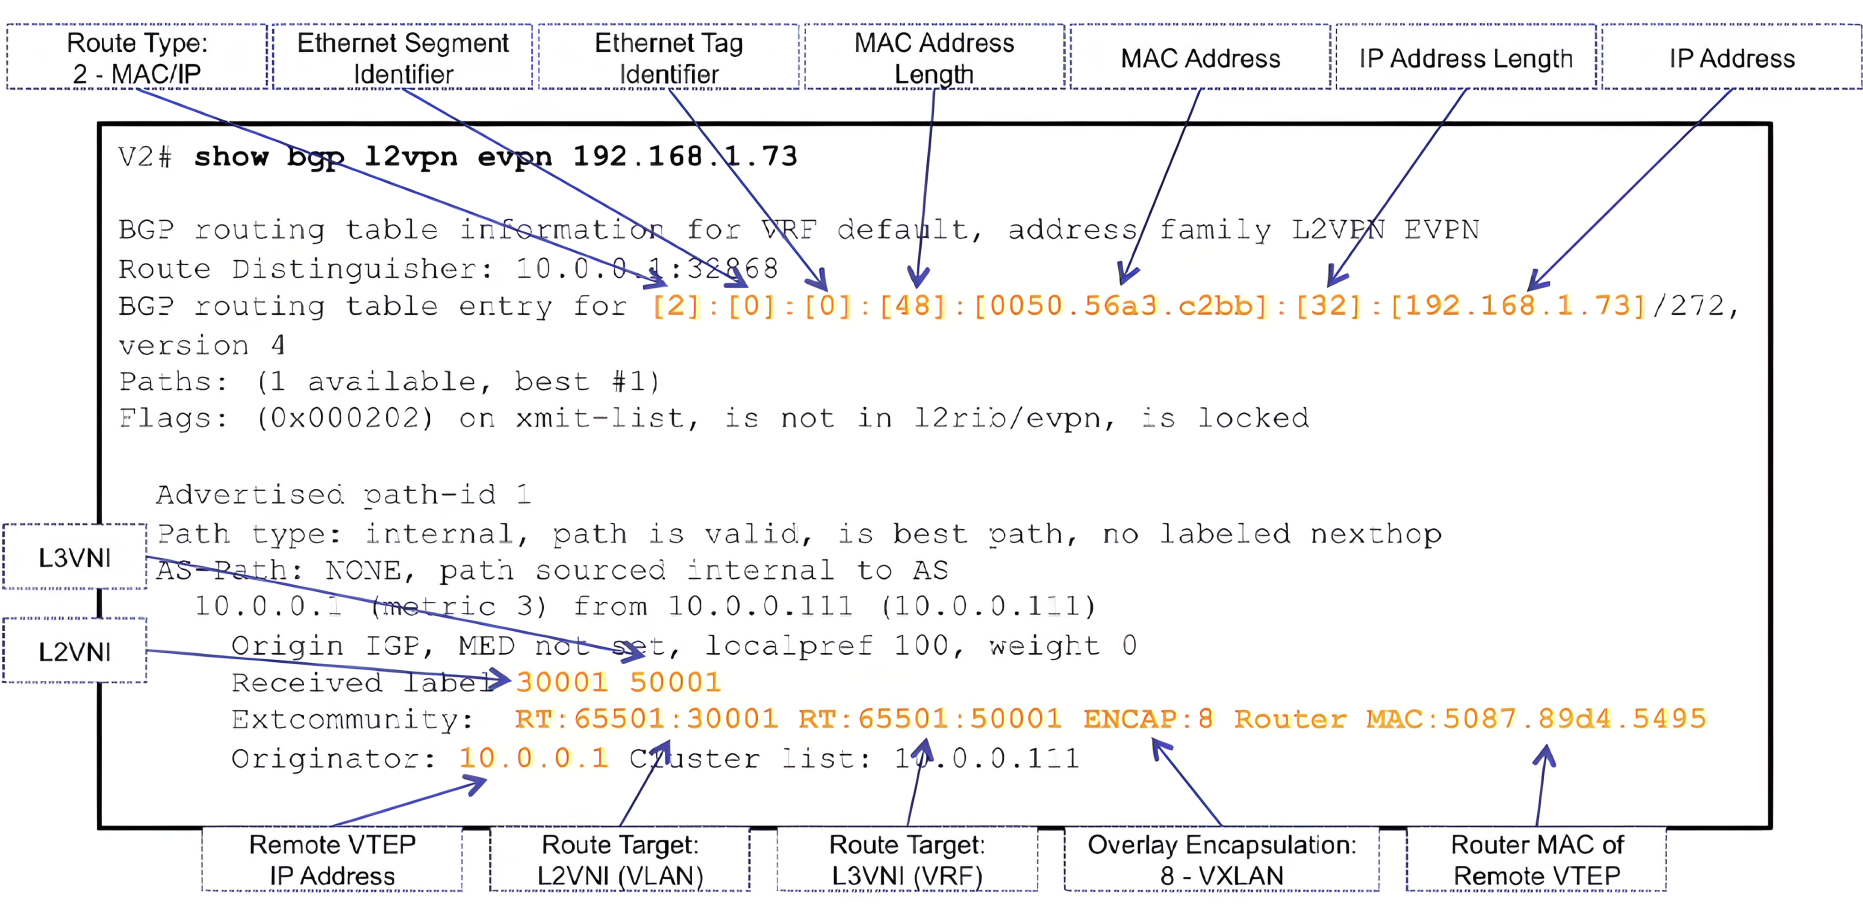
\includegraphics[width=\linewidth]{route-type-2}
			\textbf{Route Type 5:}
			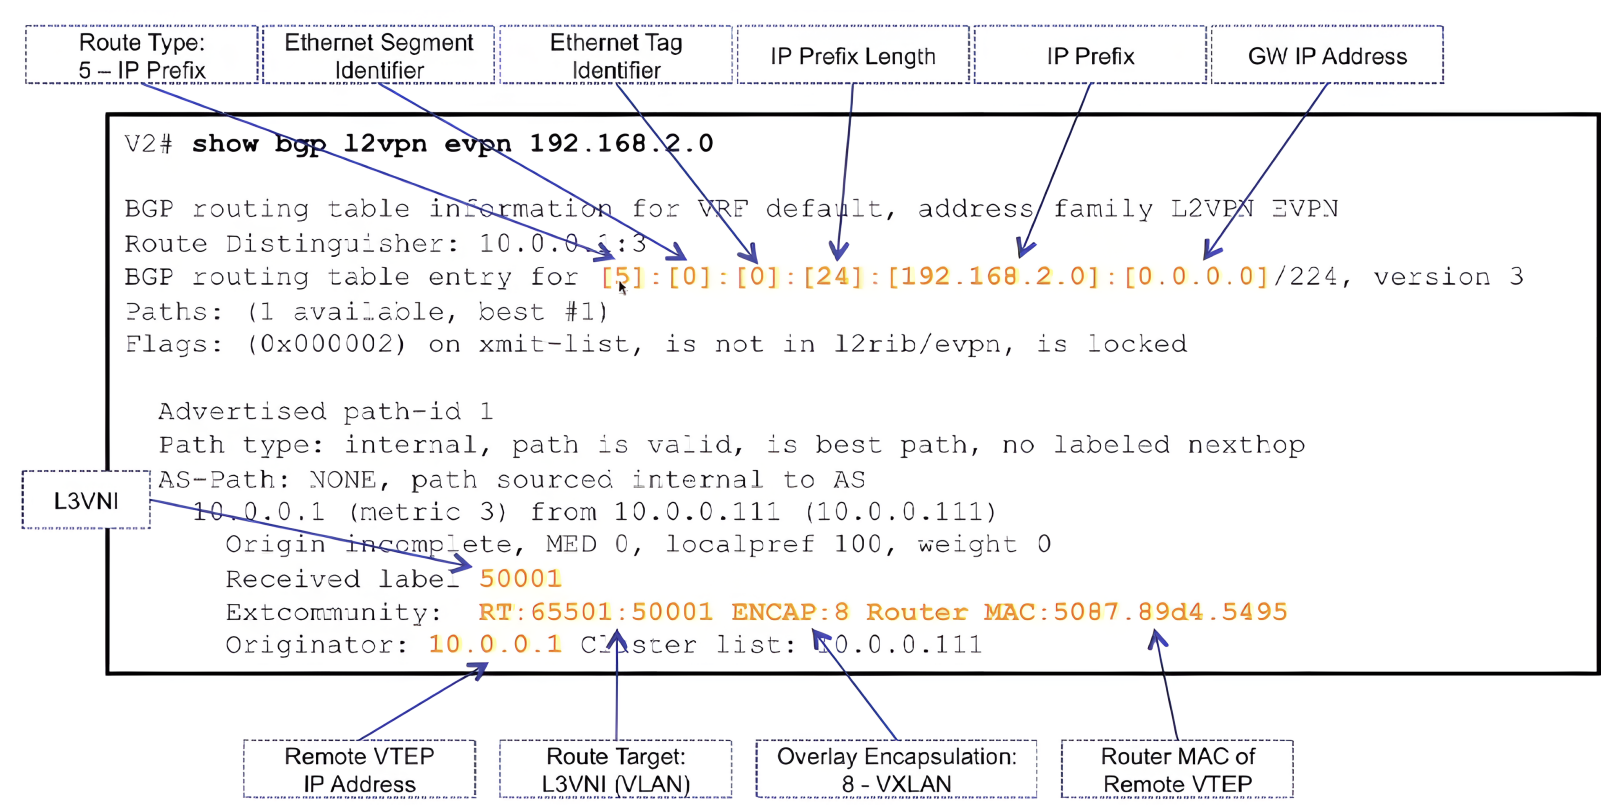
\includegraphics[width=\linewidth]{route-type-5}
		\end{center}
		\section{Prüfung Vorjahr}
		\subsection{Network design}
		\begin{itemize}
			\item \textbf{3-tier campus network}: Default Gateway (D), QoS marking (A), STP Root Port (A), HSRP, VRRP or GLBP (D), “Simple” (C), OSPF Totally Stub Area (D), High availability (C)
			\item \textbf{Campus Design}: used to reduce size of L2 domain: EVPN, MPLS
		\end{itemize}
		\subsection{Rest}
		\begin{itemize}
			\item \textbf{MP\_REACH\_NLRI:} Next hop, MAC Address
			\item VXLAN is a data plane technology which encapsulates Ethernet frames in UDP datagrams to tunnel layer 2 frames over a layer 3 network.
			\item The underlay network is unaware of VXLAN devices that connect to the physical switches are unaware of VXLAN. 
			\item A route distinguisher is used to uniquely identify a route in combination with the destination prefix.
		\end{itemize}
		\section{El Memez}
		Always space for memez ;)
		\begin{center}
			
\includegraphics[width=100px]{meme-3}
		\end{center}
		Calc
		
	\end{multicols*}
	
	% \input{./appendix.tex}
	
\end{document} 